\section{Method}
\label{sec:method}

Our method (see \autoref{fig:overview}) comprises three stages: forward rendering, detail generation, and inverse rendering discussed below. We then present our three technical contributions in Sections~\ref{sec:second-controlnet} to~\ref{sec:attention_bias}.


\paragraph{Forward rendering.}
We begin with a user-provided asset comprising of known geometry and the material to be enhanced, as well as a 3D scene providing context for the asset.
We render the scene from a small number of views (between 9 and 16 views in practice) in an orbit around the asset.
The output of the renderer consists of the renderings as well as auxiliary buffers of surface normals, which serve to condition the diffusion model during the next stage.

\paragraph{Detail generation.}

The renderings from the previous stage are passed to an off-the-shelf diffusion model to add detail to the renderings, conditioned on a text prompt and the auxiliary buffers. Although the rendered views could be enhanced individually, we find that mutual view consistency is improved if we use \emph{multi-view visual prompting}~\cite{flashtex}, in which we concatenate all views into a grid (e.g. $3\times 3$ or $4\times 4$) and enhance them simultaneously.






While multi-view prompting improves consistency across the views at a coarse scale, there remains enough variation in fine-scale detail between views to make reconstruction of highly detailed materials challenging.
To remedy this, we propose two modifications to the diffusion model:
using view-correlated input noise that is anchored in 3D space (Section~\ref{sec:noise_warping}) 
and biasing the attention layers with pixel-to-pixel correspondence information (Section~\ref{sec:attention_bias}).


\paragraph{Inverse rendering.}
We finally propagate the detail generated by the diffusion model back to the original material of the 3D asset, leveraging a differentiable renderer~\cite{mitsuba} to minimize the difference between the enhanced views and the rendered material in a stochastic gradient optimization.
In all our results, we optimize the spatially-varying albedo, normal, and roughness textures of a typical PBR material~\cite{Burley2012}, but any differentiable material definition can be used in principle.
We initialize the optimization state with the original textures; this improves the convergence likelihood. %

\begin{figure*}[htbp]
    \centering%
    \setlength{\tabcolsep}{0.002\textwidth}%
    \renewcommand{\arraystretch}{1}%
    \footnotesize%
    \begin{tabular}{ccc}
        Latent pixel correspondences
        &
        Unmodified attention scores
        &
        Biased attention scores
        \\[0.8mm]
        \begin{overpic}[width=0.332\textwidth]{figures/attnviz/correspondences_crop.jpg}
            \begin{tikzpicture}[overlay, remember picture]
                \draw[-{Stealth[length=2mm]},green,thick,] (3.50,1.25) -- (3.12,0.78);
                \draw[-{Stealth[length=2mm]},red,thick,]   (1.45,1.30) -- (1.07,0.83);
                \draw[-{Stealth[length=2mm]},red,thick,]   (5.63,1.30) -- (5.25,0.83);
            \end{tikzpicture}
        \end{overpic}
        &
        \begin{overpic}[width=0.332\textwidth]{figures/attnviz/unbiased_crop.jpg}
        \end{overpic}
        &
        \begin{overpic}[width=0.332\textwidth]{figures/attnviz/biased_crop.jpg}
            \begin{tikzpicture}[overlay, remember picture]
                \draw[-{Stealth[length=2mm]},red,thick,]   (1.45,1.30) -- (1.07,0.83);
                \draw[-{Stealth[length=2mm]},red,thick,]   (5.63,1.30) -- (5.25,0.83);
            \end{tikzpicture}
        \end{overpic}
    \end{tabular}
    \caption{
        Left:
        For one latent pixel (green), we highlight the corresponding neighborhoods in the other conditioning views in red; we use ray tracing to check for occlusions.
        Middle:
        One attention score matrix \emph{row} related to that green latent pixel can be rearranged into an image showing how much it attends to all other latent pixels in one stage of the diffusion model.
        (We crop to three views of the $3 \times 3$ grid. The supplementary document includes an uncropped version.)
        Right:
        We bias the matrix entries in \emph{columns} that correspond to the identified red regions to promote attention---and hence consistency---between these latents.
    }
    \label{fig:attention_viz}
\end{figure*}

\subsection{Structure-preserving detail enhancement}
\label{sec:second-controlnet}

To enhance the rendered views while preserving the character of the input material, we follow the approach of \citet{meng2022sdedit} and add a user-controlled amount of noise to the rendered views to get the initial state for diffusion. This is not enough, however, to preserve the original material and geometry. Hence, we additionally condition the diffusion model with two publicly available ControlNets~\cite{controlnet}: \emph{ControlNet tile}, trained to do super-resolution, which we repurpose to respect the input view while enhancing details, and \emph{ControlNet normal} that helps preserve lighting and curvature details using our auxiliary normal buffer as input.

Together with our other modifications (Sec. \ref{sec:noise_warping} and \ref{sec:attention_bias}) we find this to be effective at achieving consistency with the original material and across views, while avoiding expensive training of task-specific ControlNets as used in prior work~\cite{flashtex}.






\subsection{View-correlated noise prior}
\label{sec:noise_warping}













Although the relationship between the initial noise input and the image output in diffusion is highly non-linear, the two are correlated.
This has previously been exploited for temporal consistency by warping noise by a motion field, and we take a similar approach.
Because diffusion models are highly sensitive to the noise statistics, the noise we produce must be uncorrelated within each view and have uniform variance, or we risk significant artifacts.

Based on \citet{chang2024how}, we propose a simple method to correlate the initial noise of the diffusion model across views while preserving its statistics.
In contrast to their application, we deal with a sparse set of views that do not undergo smooth motion.
It would be challenging to warp an initial noise from a reference view due to the significant amount of disocclusion between views.
Instead, we exploit the known geometry of the asset and anchor a reference noise field in the UV space of the asset.

For each view, we then project the noise from UV space (we use $1024\times 1024$ noise textures) into image space and use this as the initial state for diffusion. Compared to the analytic integration of \citet{chang2024how}, we use a simpler but effective \emph{supersampling} approach.
We subdivide each pixel into a grid of subpixels ($4\times 4$ in our implementation) and project the corners of each subpixel into the UV space of the object:
\begin{center}
    \begin{overpic}[width=0.95\columnwidth]{figures/warped_noise/figure.pdf}
        \footnotesize
        \put(-6.4,29.1){ \begin{minipage}{2cm}\centering Subdivided\\pixel \end{minipage}}
        \put(71.7,34){   \begin{minipage}{2cm}\centering UV space zoom-in  \end{minipage}}
        \put(73,3){$A_i$\,:}
    \end{overpic}
\end{center}
We then sample the noise field at the center of each projected subpixel, and compute an area-weighted average of the sampled noise values: $\sum_i f_i \cdot A_i$, where $A_i$ is the area of each projected subpixel $i$, and $f_i$ its noise value. Neighboring pixels don't overlap and generally average distinct sets of noise texels, and the resulting noise is independent within each view.



The variance of the projected noise is highly non-uniform, depending on the projected area of each pixel.
To correct this, we could normalize the noise field by an estimate of its variance: $\sqrt{\sum_i \smash{A_i^2}}$.
However, because multiple subpixels may map to the same noise texel, we need to additionally account for the covariance between subpixels. We estimate this with $\mathrm{Cov}_i=\max(A_\mathrm{texel}/A_i-1, 0)$ where $A_\mathrm{texel}=1024^{-2}$ is the area of a noise texel. Intuitively, this counts how many times a distinct noise value is overcounted on average.
The final normalization factor is then $\sqrt{\sum_i A_i^2 (1 + \mathrm{Cov}_i)}$. This matches the variance of projected- and reference noise.

In the case of extreme magnification of the noise texture, individual noise texels may project to multiple pixels and correlate noise within the image.
This is rare and usually caused by missing or degenerate UVs, but it can negatively impact the quality of diffusion.
As a safeguard, we smoothly blend the projected noise value with independent white noise when the pixel area in UV space, $\sum_i A_i$, approaches the area of a noise texel.

















\begin{figure*}[htbp]
    \centering%
    \setlength{\tabcolsep}{0.002\textwidth}%
    \renewcommand{\arraystretch}{1}%
    \footnotesize%
    \begin{tabular}{cccccccc}
        &Initial asset& \multicolumn{6}{c}{
            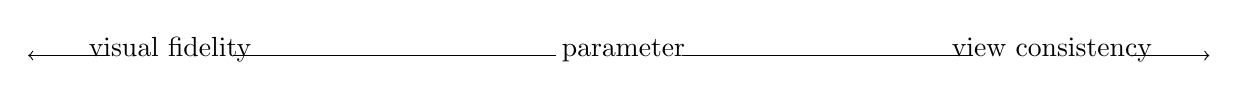
\begin{tikzpicture}
                \draw[<-] (0,0) -- (1,0);
                \draw[-] (2.6,0) -- (6.7,0);
                \draw[-] (8.3,0) -- (12,0);
                \draw[->] (14,0) -- (15,0);
                \node[above] at (1.8,-0.2) {visual fidelity};
                \node[above] at (7.5,-0.2) {$\bias$ parameter};
                \node[above] at (13,-0.2) {view consistency};
            \end{tikzpicture}
        }\\[-4pt]%
        && 0.0 & 0.6 & \textbf{1.2} & \textbf{1.8} & 2.4 & 3.0\\%
        \rotatebox{90}{\hspace*{4em}View 1}&%
        \includegraphics[height=0.14\linewidth, trim=150 0 100 0, clip]{figures/hparams_adjusting/initial_2_overlay.jpg}&%
        \includegraphics[height=0.14\linewidth, trim=200 40 300 460, clip]{figures/hparams_adjusting/0.0_2_overlay.jpg}&%
        \includegraphics[height=0.14\linewidth, trim=200 40 300 460, clip]{figures/hparams_adjusting/0.6_2_overlay.jpg}&%
        \includegraphics[height=0.14\linewidth, trim=200 40 300 460, clip]{figures/hparams_adjusting/1.2_2_overlay.jpg}&%
        \includegraphics[height=0.14\linewidth, trim=200 40 300 460, clip]{figures/hparams_adjusting/1.8_2_overlay.jpg}&%
        \includegraphics[height=0.14\linewidth, trim=200 40 300 460, clip]{figures/hparams_adjusting/2.4_2_overlay.jpg}&%
        \includegraphics[height=0.14\linewidth, trim=200 40 300 460, clip]{figures/hparams_adjusting/3.0_2_overlay.jpg}\\%
        \rotatebox{90}{\hspace*{2em}View 2, $+ 40^\circ$}&
        \includegraphics[height=0.14\linewidth, trim=150 0 100 0, clip]{figures/hparams_adjusting/initial_3_overlay.jpg}&%
        \includegraphics[height=0.14\linewidth, trim=200 40 300 460, clip]{figures/hparams_adjusting/0.0_3_overlay.jpg}&%
        \includegraphics[height=0.14\linewidth, trim=200 40 300 460, clip]{figures/hparams_adjusting/0.6_3_overlay.jpg}&%
        \includegraphics[height=0.14\linewidth, trim=200 40 300 460, clip]{figures/hparams_adjusting/1.2_3_overlay.jpg}&%
        \includegraphics[height=0.14\linewidth, trim=200 40 300 460, clip]{figures/hparams_adjusting/1.8_3_overlay.jpg}&%
        \includegraphics[height=0.14\linewidth, trim=200 40 300 460, clip]{figures/hparams_adjusting/2.4_3_overlay.jpg}&%
        \includegraphics[height=0.14\linewidth, trim=200 40 300 460, clip]{figures/hparams_adjusting/3.0_3_overlay.jpg}\\%
    \end{tabular}%
    \caption{The bias parameter $\bias$ trades between visual fidelity (left insets) and multi-view consistency (right insets). The first column shows the initial asset in two views that condition the diffusion model. The white shapes outline a UV region, which we analyze in the insets to illustrate the impact of the $\bias$ parameter on generated visuals.
    Values between 1.2 and 1.8 strike a good balance in this particular scene.}
    \label{fig:hparams}
\end{figure*}










\subsection{Pixel-correspondence attention bias}
\label{sec:attention_bias}

The second technique for improving the multi-view consistency amounts to biasing the self-attention mechanism of the diffusion model according to a reprojection prior.

As described in Section~\ref{sec:background}, the self-attention modules allow image regions to influence each other.
We refer to these regions as \emph{latent pixels} to emphasize that they map to pixels in the input/output image.
The $\matQ \matK^\top$ product in the self-attention module forms a large $N \times N$ score matrix where entry $[i \in Q,j \in K]$ describes how strongly latent pixel $i$ attends to latent pixel $j$; $N$ is the total number of latent pixels.

Our goal is to increase the attention scores between latent pixels in different views that observe the \emph{same surface patch}.
This will increase the chance that these latent pixels will denoise to consistent visuals in the resulting images.
Conceptually, we construct an $N\times N$ \emph{bias matrix} $\matB$,
where any positive value $\matB[i,j]$ will boost the attention of pixel $i$ to pixel $j$.

We determine the values of $\matB$ as follows.
For each pair of pixels $i$ and $j$ (where $i \neq j$) in the $3\times3$ latent image grid,
we cast a ray through the center of latent pixel $j$ into the 3D scene, finding the first hit point~$\mathbf{p}$.
We then project $\mathbf{p}$ onto the image plane containing pixel $i$ and check that $\mathbf{p}$ and the projection $\mathbf{q}$ are mutually visible.
\begin{center}
    \begin{overpic}[width=0.95\columnwidth]{figures/pixel_correspondence/figure.pdf}
        \footnotesize
        \put(53.5,15.2){$\mathbf{p}$}
        \put(18.5,14.7){$\mathbf{q}$}
        \put(29.0,34.5){Latent pixel $i$}
        \put(54.0,32.0){Latent pixel $j$}
        \put(60.0,14.9){\rotatebox{7}{$\matB[i,j_0\!] \!=\! \bias$}}
        \put(61.0, 6.3){\rotatebox{7}{$\matB[i,j_1\!] \!=\! 0$}}
        \put(11.0,19.0){$\mathcal{I}$}

    \end{overpic}
\end{center}
If the projection $\mathbf{q}$ is within a neighborhood $\mathcal{I}$ of pixel $i$, we set the value in the bias matrix to a user-defined constant: $\matB[i,j] = \bias$.


The matrix is used to alter the attention operation as:
\[
\text{Attention}(\matQ, \matK, \matV) = \text{softmax}\left(\frac{\matQ \matK^\top + \matB}{\sqrt{d_k}}\right)\matV.
\]
In practice, constructing the full $N \times N$ matrix is often prohibitive, and the bias term has to be evaluated on the fly (see Sec. \ref{sec:implementation}).

The U-Net applies self-attention at multiple scales, and we adjust the size of neighbordhood $\mathcal{I}$ ($9^2, 5^2, 3^2, 1^2$ for layers 1-4, respectively) to map to the same size patch in the original image. Figure \ref{fig:attention_viz} visualizes exemplary attention scores before and after adding the bias for a single specific surface point. The increment $\bias$ is a user-defined constant analysed in Figure~\ref{fig:hparams}. Increasing $\bias$ improves view consistency but eventually generates less compelling appearance as the diffusion starts to lose its global view of the image.












    










    

    


    






    















    




